\documentclass{beamer}
\usepackage[utf8]{inputenc}
\usepackage[spanish]{babel}
\usepackage{hyperref}
\usepackage{verbatim}
\usepackage{listings}
\usepackage{tikz}
\usepackage{ulem}
\usetikzlibrary{arrows}

\setbeamercovered{invisible}
\usetheme{Frankfurt}
\usefonttheme{serif}

% Configurar los listings (Códigos)
\renewcommand{\lstlistingname}{Código}
\lstset{
	language=C++,               % Lenguaje
	basicstyle=\ttfamily\tiny,  % Tipo de fuente
	keywordstyle=\color{blue},  % Color de palabras clave
	stringstyle=\color{red},    % Color de strings
	commentstyle=\color{gray},  % Color de comentarios
	showstringspaces=false,     % No muestrar el _ cuando el string tiene espacios
	breaklines = true,          % Partir las líneas largas
	breakatwhitespace=true,	    % Partir las líneas en un espacio
	numbers=left,				% Numerar las líneas a la izq
	numberstyle=\tiny,			% Poner los números de las líneas pequeños
	numberblanklines=true,      % Numerar las líneas en blanco
	columns=fullflexible,       % No perder el formato al dejar los espacios
	keepspaces=true,   			% Dejar los espacios insertados
	frame=tb,					% Poner el recuadro
}


\title{Desarrollo e implementación de un programa de trabajo para el semillero de programación}
\author{Por: \\ Ana Echavarría Uribe \\ \quad \\ Tutor: \\ Juan Francisco Cardona Mc'Cormick}

\institute{Universidad EAFIT}
\date{15 de marzo de 2013}

\begin{document}

\begin{frame}
	\titlepage
\end{frame}

\begin{frame}
	\frametitle{Contenido}
	\tableofcontents
\end{frame}

\section{Problema}
	\begin{frame}
		\frametitle{Problema}
		\begin{itemize}
			%\item El semillero de programación busca enseñar nuevas técnicas de programación a estudiantes interesados en esta área.
			\item Se preparan los alumnos para participar en las maratones de programación realizadas por ACIS/REDIS y por la ACM-ICPC.
			\item El semillero ha estado a cargo de alumnos destacados en las maratones de programación.
			\item No se ha desarrollado nunca un plan de trabajo para el curso.
		\end{itemize}		
	\end{frame}
	
	\begin{frame}
		\frametitle{Objetivo General}
			\begin{block}{}
			Desarrollar e implementar un plan de actividades y temas de fundamentación matemática para el semillero de programación que busque mejorar las habilidades de programación de los estudiantes, basándose en la metodología usada por Steven Halim en el curso Competitive Programming de la Universidad Nacional de Singapur y en otras que en el desarrollo del proyecto puedan surgir.
			\end{block}
	\end{frame}

\section{Curso Competitive Programming}
	\begin{frame}
		\frametitle{Steven Halim}
		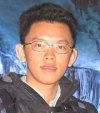
\includegraphics[height = 0.25\textheight]{halim.jpg}
		\begin{itemize}
			\item{Profesor de la Universidad Nacional de Singapur (UNS)}
			\item{Doctor en computación de la UNS}
			\item{Co-autor de los libros Competitive Programming 1 y 2}
			\item{Profesor del curso Competitive Programming en la NUS}
			\item{Entrenador del equipo de programación (ACM-ICPC) de la NUS y del equipo de la IOI de Singapur}
		\end{itemize}
	\end{frame}
	
	\begin{frame}
		\frametitle{Competitive Programming @ NUS}
		% \includegraphics[height = 0.25\textheight]{book.jpeg}
		\begin{itemize}
			\item{Curso creado en 2008 que busca fortalecer las habilidades de programación de sus estudiantes destacados para prepararlos para las competencias universitarias de programación de la ICPC}
			\item{Enfocado a estudiantes de tercer año con buenas habilidades de programación}
			\item{Curso avanzado, cubre muchos temas en poco tiempo}
			\item{Material abierto al público en \url{https://sites.google.com/site/stevenhalim/home/material}}
			\item \Large{\sout{Exámenes} $\rightarrow$ Competencias}
		\end{itemize}	
	\end{frame}

\section{Semillero de programación}
	\begin{frame}
		\frametitle{Semillero de programación - Eafit}
		\begin{itemize}
			\item Estudiantes interesados en mejorar sus habilidades de programación y competir en las maratones
			\item Estudiantes en su mayoría de 1ro y 3er semestre
			\item No tienen conocimiento previo de C++
			\item Reuniones semanales de 2 horas
		\end{itemize}
		
		\begin{center}
			\begin{tikzpicture}
				\draw [line width=3, ->] (0,0) -- (0,-1.1);
			\end{tikzpicture}\\
			\large{El semillero va más lento que el curso de la NUS} 
		\end{center}
	\end{frame}
	
	\begin{frame}
		\frametitle{Temas vistos}
		\begin{enumerate}
			\item{Introducción a los jueces de programación}
			\item{Introducción a C++ y a métodos de entrada y salida de datos}
			\item{Arreglos y Vectores en C++}
			\item{Representación de grafos: dirigidos, no dirigidos y con pesos}
			\item{Estructuras de datos: pila, cola, mapa, set y heap}
			\item{Recorrido de grafos: DFS y BFS}
			\item{Ordenamiento Topológico y Componentes Fuertemente Conexas}
			\item{Algoritmo de Dijkstra}
		\end{enumerate}
	\end{frame}
	
	\begin{frame}
		\frametitle{Problemas propuestos}
		\begin{itemize}	
			\item Luego de explicar cada tema se dejan como tarea un conjunto de problemas que apliquen los temas aprendidos.\\
			\item Los problemas de las competencias se escogen de los problemas propuestos en el libro de Steven Halim.\\
			\item Se resuelven los problemas antes de proponérselos como ejercicio a los estudiantes.
		
		\end{itemize}
	\end{frame}
	
	\begin{frame}{Competencias}
		\begin{itemize}
			\item Al igual que en el curso de la NUS, se hacen competencias competencias con los problemas propuestos.
			\item Las competencias se hacen utilizando el sitio \url{http://contests.factorcomun.org/}\\
			\item Estas comienzan al acabar la reunión y terminan al inicio de la siguiente, donde se discuten y resuelven los problemas.\\
			\item Con las competencias se mide el nivel de los estudiantes, esto permite ajustar el nivel de los temas.
		\end{itemize}
	\end{frame}
	
	
	\begin{frame}
		\frametitle{Competencias}
		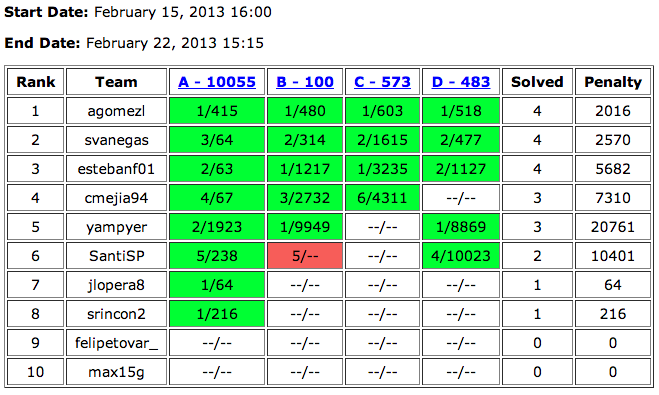
\includegraphics[width = 0.95\textwidth]{contest.png}
	\end{frame}
	
	\begin{frame}
		\frametitle{Competencias}
		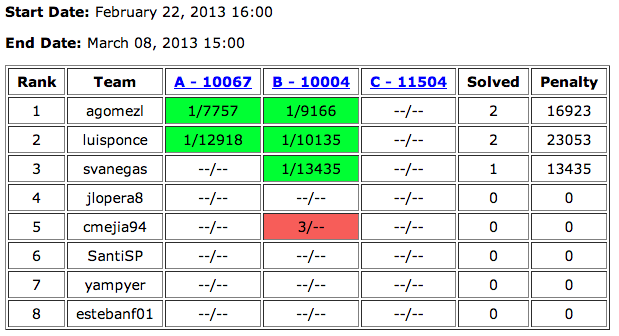
\includegraphics[width = 0.95\textwidth]{contest2.png}
	\end{frame}

% \section{Bibliografía}
% 	\begin{frame}[allowframebreaks]
% 		\frametitle{Bibliografía}
% 		\bibliographystyle{plain}
% 		\bibliography{Biblio}
% 	\end{frame}
	
\section{Preguntas}
	\begin{frame}
		\frametitle{Preguntas}
		
\includegraphics[width = 0.9\textwidth]{preguntas.jpeg}
	\end{frame}

\end{document}